\chapter{Variation Reduction Methods}
\label{cap:variation_reduction}

Results of Monte Carlo simulations are always estimates with a margin of error. \emph{Variance Reduction Techniques} (VRTs) are a set of
mathematical strategies designed to make that estimate more precise (reducing the "noise" or variance) without requiring millions of additional, computationally expensive simulations.
	
Think of it like trying to determine the average height of people in a city. You could either: pick 100 people completely at random (standard method), or pick 50 people at random, 
but for every tall person you pick, you intentionally pick a short person to balance the scale (VRT method). The second approach reaches the "true" average much faster because
you've manually removed the extreme outliers that skew the results.
	
When you simulate a complex model like Vasicek or GBM, "raw" Monte Carlo is often too slow or jittery for real-time risk management. VRTs  allow you to achieve the same level of accuracy with smaller effort.

Some of the most popular variation reduction techniques will be described in this Chapter:
	
\begin{itemize}
	\tightlist
	\item Antithetic Variates
	\item Control Variates
	\item Importance Sampling
\end{itemize}
	
As we have seen the standard error of a Monte Carlo estimate is given by: $\text{standard error} = \frac{\sigma}{\sqrt{N}}$. To cut the error in half using the standard method, you need 4 times
more paths ($N$). With Variance Reduction, instead of increasing $N$, you focus on shrinking $\sigma$ (the numerator) through clever sampling, which is often much more efficient for high-performance
banking systems.
	
\section{Antithetic Variates}
\label{sec:monte-carlo-with-antithetic-variates}
	
\emph{Antithetic Variates} is a powerful \textbf{variance reduction} technique used in Monte Carlo simulations to improve computational efficiency and precision. The core idea is to introduce a deliberate
negative correlation between pairs of simulated paths. 

For every random sample $Z$ drawn from a standard normal distribution to generate a path, a second "mirror" path is generated using $-Z$. By averaging these two complementary observations, the terms with high
positive variance tend to cancel out those with high negative variance. Mathematically, this reduces the standard error of the estimate because the covariance between the two paths is negative, leading to a faster
convergence toward the true value compared to using twice as many independent random draws.
	
Technically, the Antithetic Variates technique can be used for any distribution, but it is most effective and straightforward when the distribution is symmetric around a mean.
	
While the \emph{normal distribution} is the most common use case (especially in finance), the principle relies on the probability integral transform, see Sec.~\ref{sec:distribution-transformation}.

\paragraph{Symmetric Distributions}: if a distribution is symmetric around its mean $\mu$, you can generate antithetic paths directly. If you sample $X$, your antithetic sample is $X'=2\mu -X$ 
(in the case of a Standard Normal $\mathcal{N}(0,1)$, this simplifies to $X'=-X$).

\paragraph{Non-Symmetric Distributions}: even if a distribution is not symmetric, you can still use the technique. This is because almost all random variables are generated by transforming a Uniform distribution $\mathcal{U}(0,1)$. The "mirroring" happens at the Uniform level: generate a random number $u$ from $\mathcal{U}(0,1)$, use $1-u$ as your antithetic sample, transform both ($u$ and $1-u$) into your target
distribution using the Inverse Cumulative Distribution Function ($F^{-1}$).

As an example let's see how to simulate an exponential distribution. Its CDF is: $F(x)=1-e^{-\lambda x}$. To sample, we set $F(x)=u$ (where $u$) is a random uniform number
between 0 and 1). Solving for x: 
\begin{equation}
	\begin{gathered}
		u=1-e^{-\lambda x} \\
		1-u=e^{-\lambda x} \\
		\ln(1-u)=-\lambda x \\
		x=-\ln(1-u)/\lambda
	\end{gathered}
\end{equation}

Finally you take $X=\frac{-\ln(u)}{\lambda}$ and $X'=\frac{-\ln(1-u)}{\lambda}$. These two values will be negatively correlated, successfully reducing variance.
	
The effectiveness of Antithetic Variates depends on the function you are simulating being monotonic. If the function is not or if the variance of the average of the pairs is higher than the variance of the individual
samples, the technique fails. The mathematical condition for success can be expressed as 

\begin{equation}
\var(f(U))+\var (f(1-U))+2\cov (f(U),f(1-U))]
\end{equation}
	
This occurs only if $\cov(f(U),f(1-U))<0$ (negative correlation). In the $x^2$ example: Since $(x)^2=(-x)^2$, the correlation is +1, which actually maximizes the estimate variance instead of reducing it.
	
This example shows the use of antithetic variates for estimating the mean and standard error of two different functions: $X^2$ and $e^{X/2}$, where $X$ follows a standard normal distribution.

\begin{ipythonnon}
import numpy as np
import matplotlib.pyplot as plt

def simulate_exp2(n_samples):
	x1 = np.random.randn(n_samples)
	x2 = -x1
	x_std = np.random.randn(n_samples*2)
	return np.exp(x1/2), np.exp(x2/2), np.exp(x_std/2)

def simulate_x2(n_samples):
	x1 = np.random.randn(n_samples)
	x2 = -x1
	x_std = np.random.randn(n_samples*2)
	return np.power(x1, 2), np.power(x2, 2), np.power(x_std, 2)

def simulate_exponential(n_samples, rate=1.0):
	u = np.random.uniform(0, 1, n_samples // 2)
	u_antithetic = 1 - u
	x1 = -np.log(u) / rate
	x2 = -np.log(u_antithetic) / rate
	x_std = -np.log(np.random.uniform(0, 1, n_samples)) / rate    
	return x1, x2, x_std

def analysis(x1, x2, x_std):
	anti_mean = (x1 + x2) / 2
	std_mean = x_std.reshape(-1, 2).mean(axis=1)
	
	print(f"Variance (Standard MC): {np.var(std_mean):.6f}")
	print(f"Variance (Antithetic):  {np.var(anti_mean):.6f}")
	print(f"Reduction: {100*(1-np.var(anti_mean)/np.var(std_mean)):.2f}%")

N = 20000
x1, x2, x_std = simulate_exponential(N)
analysis(x1, x2, x_std)	

x1, x2, x_std = simulate_x2(N)
analysis(x1, x2, x_std)

x1, x2, x_std = simulate_exp2(N)
analysis(x1, x2, x_std)
\end{ipythonnon}
\begin{ioutput}
Variance (Standard MC): 0.181873
Variance (Antithetic):  0.038561
Reduction: 78.80%
Variance (Standard MC): 1.012585
Variance (Antithetic):  2.014346
Reduction: -98.93%
Variance (Standard MC): 0.506297
Variance (Antithetic):  0.183833
Reduction: 63.69%
\end{ioutput}
	
\subsection{European Call Option with Antithetic Variates}
\label{sec:monte-carlo-european-call-option-with-antithetic-variates}
	
Here we implement a Monte Carlo simulation to price a European call option, incorporating the antithetic variates technique for variance reduction.
	
\begin{ipythonnon}
import numpy as np
from scipy.stats import norm

def mc_comparison(S0, K, r, T, sigma, n):
	A = (r - 0.5 * sigma**2) * T
	B = sigma * np.sqrt(T)
	discount = np.exp(-r * T)
	
	Z = np.random.randn(n)
	payoff_a1 = np.maximum(0, S0 * np.exp(A + B * Z) - K)
	payoff_a2 = np.maximum(0, S0 * np.exp(A + B * (-Z)) - K)
	
	E_antithetic = discount * 0.5 * (payoff_a1 + payoff_a2)
	price_anti = np.mean(E_antithetic)
	se_anti = np.std(E_antithetic) / np.sqrt(n)
	
	Z_std = np.random.randn(2 * n)
	payoff_std = discount * np.maximum(0, S0 * np.exp(A + B * Z_std) - K)
	
	price_std = np.mean(payoff_std)
	se_std = np.std(payoff_std) / np.sqrt(2 * n)
	
	return (price_anti, se_anti), (price_std, se_std)

S0, K, r, T, sigma, n = 100, 100, 0.05, 1, 0.2, 10000

(p_anti, s_anti), (p_std, s_std) = mc_comparison(S0, K, r, T, sigma, n)

print(f"Antithetic: Price = {p_anti:.4f}, Std Error = {s_anti:.6f}")
print(f"Standard:   Price = {p_std:.4f}, Std Error = {s_std:.6f}")
print(f"Variance Reduction: {100*(1-(s_anti**2/s_std**2)):.2f}%")
\end{ipythonnon}	
	
\begin{ioutput}
Antithetic: Price = 10.6164, Std Error = 0.074618
Standard:   Price = 10.5487, Std Error = 0.104660
Variance Reduction: 49.17%
\end{ioutput}
	
Try to guess what would be the outcome of a similar simulation involving a \emph{Straddle} option (a bet on volatility), whose payoff $V$ is $|S_T - K|$.
	
\section{Control Variates}

Control Variates is a variance reduction technique that improves the precision of a Monte Carlo simulation by leveraging the known solution of a simpler, related problem.

In this approach, instead of simulating only the target asset (the "unknown"), you simultaneously simulate a "control" variable whose expected value is already known analytically. 
By observing how the simulated control variable deviates from its true theoretical value, you can apply a correction to the target simulation.

For instance, when pricing a complex Asian option, a practitioner might use a standard European option as the control variate. If the European simulation happens to overestimate the 
price due to random noise, the Asian estimate is adjusted downward by a proportional amount. This "error correction" significantly narrows the confidence intervals, allowing for 
high-precision results with far fewer paths.

Mathematically, the Control Variates technique is rooted in the property of the variance of a sum. When you add a "control" to your estimator, you are effectively performing a linear regression on the noise.
Here is the step-by-step mathematical breakdown. 

Suppose we want to estimate $\mu =\mathbb{E}[Y]$ (e.g., the expected payoff of a complex option). We find another variable $X$ (the control) where we already know the true expected value
$\mu_X=\mathbb{E}[X]$ analytically. We define a new estimator, $Y_{CV}$: 
\begin{equation}
Y_{CV}=Y+c(X-\mathbb{E}[X])
\end{equation}

Notice that $Y_{CV}$ is an unbiased estimator because if you take the expectation of both sides: 
\begin{equation}
\mathbb{E}[Y_{CV}]=\mathbb{E}[Y]+c(\mathbb{E}[X]-\mathbb{E}[X])=\mathbb{E}[Y]
\end{equation}

The goal is to choose a constant $c$ that makes $\var(Y_{CV})$ as small as possible. The variance of our new estimator is:
\begin{equation}
\var(Y_{CV})=\var(Y+cX)=\var(Y)+\var(X)+2c\cov(Y,X)
\end{equation}

To find the minimum, we take the derivative with respect to $c$ and set it to zero: 
\begin{equation}
\frac{d\var(Y_{CV})}{dc} = 2c\var(X)+2\cov(Y,X)=0
\end{equation}

Solving for $c$: 
\begin{equation}
c^*= -\frac{\cov(Y,X)}{\var(X)}
\end{equation}

If we plug this optimal $c^*$ back into the variance equation, we get the minimum variance: 
\begin{equation}
\var(Y_{CV})=\var(Y)-\frac{\cov(Y,X)^2}{\var(X)}=\var(Y)(1-\rho_{XY}^2)
\end{equation}
where $\rho_{XY}$ is the correlation coefficient between your target $Y$ and your control $X$. If $\rho =1$ (perfect correlation), the variance becomes zero. If $\rho =0$ (no correlation), the variance
remains $\var(Y)$. Even a moderate correlation (e.g., 0.9) results in a $1-0.92=19\%$ residual variance, meaning an 81\% reduction.
	
\subsection{European Call Option with Control Variates}
\label{sec:monte-carlo-european-call-option-with-control-variates}
	
Here we will see a Monte Carlo simulation to price a European call option using the control variates technique for variance reduction.
	
\begin{ipythonnon}	
import numpy as np

def mc_control_variate(S0, K, r, T, sigma, n):
	dt = T
	drift = (r - 0.5 * sigma**2) * dt
	vol = sigma * np.sqrt(dt)
	discount = np.exp(-r * T)
	
	Z = np.random.randn(n)
	ST = S0 * np.exp(drift + vol * Z)
	
	Y = discount * np.maximum(0, ST - K)
	
	X = discount * ST
	E_X = S0 
	
	cov_matrix = np.cov(Y, X)
	c = -cov_matrix[0, 1] / cov_matrix[1, 1]
	
	Y_cv = Y + c * (X - E_X)
	
	price_cv = np.mean(Y_cv)
	se_cv = np.std(Y_cv) / np.sqrt(n)
	
	price_std = np.mean(Y)
	se_std = np.std(Y) / np.sqrt(n)
	
	return (price_cv, se_cv), (price_std, se_std)

S0, K, r, T, sigma, n = 100, 105, 0.05, 1, 0.2, 20000

(p_cv, s_cv), (p_std, s_std) = mc_control_variate(S0, K, r, T, sigma, n)

print(f"Standard MC: {p_std:.4f} (SE: {s_std:.6f})")
print(f"Control Var: {p_cv:.4f} (SE: {s_cv:.6f})")
print(f"Variance Reduction: {100*(1-(s_cv**2/s_std**2)):.2f}%")	
\end{ipythonnon}
\begin{ioutput}
Standard MC: 8.0789 (SE: 0.093061)
Control Var: 7.9719 (SE: 0.042260)
Variance Reduction: 79.38%
\end{ioutput}
	
\section{Importance Sampling}
\label{sec:importance-sampling}

Assume we want to calculate the expectation $\mathbb{E}[f(X)] = \int_{-\infty}^\infty f(x)p(x)dx$ where $p(x)$ is the probability density function associated to $X$.

We can approximate this expectation using numerical approximation by sampling $n$ random values from the distribution $p$ and then calculate the sample mean:
\begin{equation}
\bar{f}(x) = \frac{1}{n}\sum_i f(x_i)
\end{equation}

The idea behind \textbf{importance sampling} is to use a simple re-formulation trick and write the expectation as
\begin{equation}
\mathbb{E}[f(X)] = \int_{-\infty}^\infty f(x)\frac{p(x)}{q(x)}q(x)dx
\end{equation}
giving the expectation of $f(x)p(x)/q(x)$ over the distribution $q$. And with that, allowing us to calculate the sample mean by sampling from $q$:
\begin{equation}
\bar{f}(x) = \frac{1}{n}\sum_i f(x_i)\frac{p(x)}{q(x)}
\end{equation}

\section{Variance Reduction}
\label{variance-reduction}

The variance of the standard Monte Carlo estimator is given by:
\begin{equation}
\frac{1}{n}\var[f(x)] = \frac{1}{n}\mathbb{E}[(f(X)-\mathbb{E}[f(X)])^2]
\end{equation}

The variance for the reformulated importance sampling estimator is:
\begin{equation}
\frac{1}{n}\var\left[\frac{p(x)}{q(x)}f(x)\right]
\end{equation}

This give us a hint on how to find a way to reduce the variance. And indeed it is relatively easy to see that this variance could be reduced to 0 by choosing $q$ as:
\begin{equation}
	\begin{split}
		q(x) = \frac{f(X)p(x)}{\mathbb{E}[f(X)]} &\implies \frac{1}{n}\var[\mathbb{E}[f(X)]] = \frac{1}{n}\mathbb{E}[(\mathbb{E}[f(X)]-\mathbb{E}[\mathbb{E}[f(X)]])^2] \\
		&= \frac{1}{n}\mathbb{E}[(\mathbb{E}[f(X)]-\mathbb{E}[f(X)])^2] = 0
	\end{split}
\end{equation}

Naturally, we don't know $\mathbb{E}[f(X)]$, as the reason we are doing this sampling after all is to find the expectation of $f$.

However, we can think of the denominator of the previous expression as some normalisation constant, and consider to construct $q$ such that it has \textbf{high} density wherever $f(x)p(x)$ is \textbf{high}.

\subsubsection{A Practical Example}

For the sake of demonstration, we choose $f=\mathcal{N}(5, 1)$, and the probability distribution $p=\mathcal{N}(9,2)$ which do not overlap too well, see Fig.~\ref{fig:importance_sampling_1}.
\begin{ipythonnon}
import numpy as np
import matplotlib.pyplot as plt

from scipy.stats import norm

f = norm(5, 1)
p = norm(9, 2)
\end{ipythonnon}

\begin{figure}[htb]
	\centering
	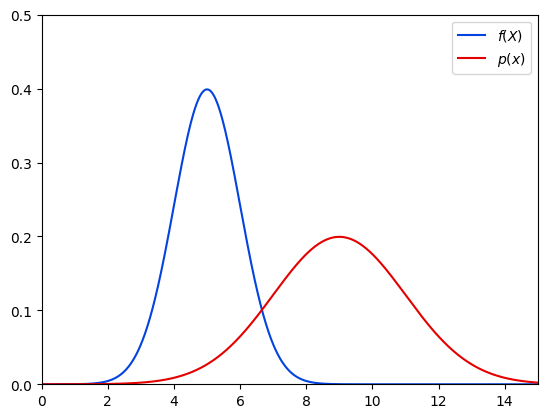
\includegraphics[width=0.7\textwidth]{figures/importance_sampling_1}
	\caption{$f$ and $p$ distributions used in the example.}
	\label{fig:importance_sampling_1}
\end{figure}

To approximate numerically the expectation, as stated above, we would now sample values $x_i$ from the distribution $p$, and compute the mean of $f(x_i)$.

Intuitively one can see why sampling from this distribution is a bad idea: for most values sampled from $p$, $f$ will be close to 0, but for a few sampled values $f$ will be very large, thus we obtain a
large variance.
\begin{ipythonnon}
N = 10000
samples = p.rvs(size=N)
f_sampling = f.pdf(samples)
mean = f_sampling.mean()
variance = f_sampling.var()

print (f"Numerical Simulation: mean {mean:.5f}, variance {variance:.5f}")
\end{ipythonnon}
\begin{ioutput}
Numerical Simulation: mean 0.03578, variance 0.00767
\end{ioutput}

Figure~\ref{fig:importance_sampling_2} (left) shows the distribution of the simulation results, there is a huge peak at 0, while the non-zero events are spread up to 0.4 leading to a large variance.

Therefore, as outlined above, we now try a new distribution $q = \mathcal{N}(5.8, 1)$, which satisfies the criterion that its PDF is high in regions where $f(x)p(x)$ is high.

\begin{figure}[htb]
	\centering
	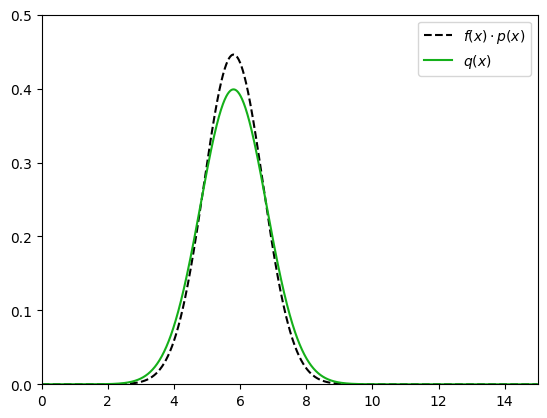
\includegraphics[width=0.7\textwidth]{figures/importance_sampling_3}
	\caption{Distribution of function $q$ to be used in the importance sampling example. Notice how it is non-zero in the relevant region $f(x)p(x) \gg 0$.}
	\label{fig:importance_sampling_3}
\end{figure}

\begin{ipythonnon}
samples2 = q.rvs(size=N)
f_sampling2 = f.pdf(samples2)*p.pdf(samples2)/q.pdf(samples2)
mean2 = f_sampling2.mean()
variance2 = f_sampling2.var()

print (f"Numerical Simulation: mean {mean:.5f}, variance {variance:.5f}")
print (f"Importance Sampling: mean {mean2:.5f}, variance {variance2:.5f}")
\end{ipythonnon}
\begin{ioutput}
Numerical Simulation: mean 0.03581, variance 0.00760
Importance Sampling: mean 0.03602, variance 0.00003
\end{ioutput}

Figure~\ref{fig:importance_sampling_2} (right) shows the distribution of the the simulation results, now the data is much more condensed around the mean leading to a much lower variance.
Looking at the numerical results we achieved a reduced variance by a factor of 200,  still with the correct mean (and the same number of samples).

\begin{figure}[htb]
	\centering
	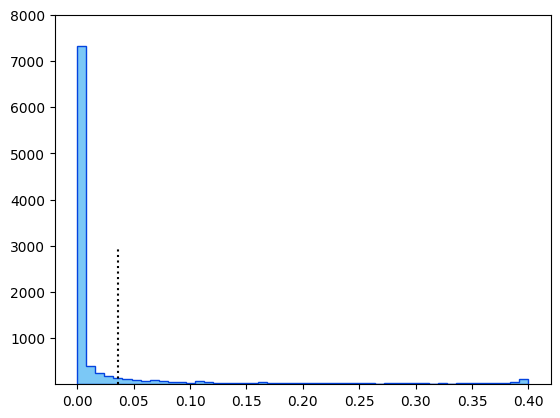
\includegraphics[width=0.45\textwidth]{figures/importance_sampling_2}
	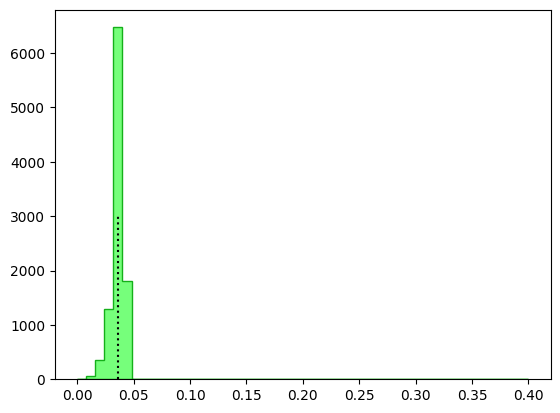
\includegraphics[width=0.45\textwidth]{figures/importance_sampling_4}
	\caption{The distribution of simulated results with standard Monte Carlo (left) and with importance sampling Monte Carlo (right). The dashed line represents the mean.}
	\label{fig:importance_sampling_2}
\end{figure}

\textbf{Note} it's not trivial to find $q$, and certainly there are much more difficult real-word scenarios. For this example I actually plotted $p(x)f(x)$ and then picked a $q$ which resembled it best.

\subsubsection{How unlucky is a 25 standard deviation return ?}
\label{sec:how-unlucky-is-a-25-standard-deviation-return}

Imagine you want to estimate the following probability:
\begin{equation}	
\theta := P(X\geq 25) = \mathbb{E}[\mathbbm{1}_{X\geq 25}]  \quad\text{where } X\sim \mathcal{N}(0, 1)
\end{equation}

The standard Monte Carlo approach proceeds as follows: generate $(X_1, X_2, \ldots ,X_n$ i.i.d. $\mathcal{N}(0,1)$; set $\mathbbm{1}_j=\mathbbm{1}_{X_j\geq 25}$ for $j=1,\ldots ,n$, set
$\hat{\theta}=\sum_{j=1}^n \mathbbm{1}_j/n$, compute approximate 95\% c.l. as $\hat{\theta}_n\pm 1.96\hat{\sigma}_n/\sqrt{n}$.

Why is this a bad idea ? Beyond knowing that $\theta$ is very small, do we even care about estimating $\theta$ accurately ?

\begin{ipythonnon}
import numpy as np
M = 1000000
Z = np.random.normal(size=M)

# Indicator function, count number of sampled variables above 25
ZT = np.where(Z>25, 1, 0)
X = np.mean(ZT)

# Calculate standard error and 95% Condifence intervals
sigma = np.std(ZT)
SE = sigma/np.sqrt(M)
CIs = [X-SE*1.96, X+SE*1.96]

print (X)
print(f'95% Confidence Level. Returns are [{CIs[0]:0.3e}, {CIs[1]:0.3e}]')
\end{ipythonnon}
\begin{ioutput}
0.0
95\% Confidence Levels. Returns are [0.000e+00, 0.000e+00]
\end{ioutput}

We have got 0 because not even one "simulation" returned a value larger than 25. So it would be better to say that the result is \textbf{undefined}.
Starting today and simulating 1 million experiments per second, most likely our Sun will be dead well before we have got a non-zero result from our MC.

Using the importance sampling technique instead we can improve our estimate giving a meaningful result.

Let's write 
\begin{equation}
	\begin{aligned}
		\theta &= \mathbb{E}[\mathbbm{1}_{\{X\geq 25\}}] = \int_{-\infty}^{\infty}\mathbbm{1}_{\{X\geq 25\}}\cfrac{1}{\sqrt{2\pi}}\exp{\left(-\frac{x^2}{2}\right)}dx = \\
		&= \int_{-\infty}^{\infty}\mathbbm{1}_{\{X\geq 25\}} \left(
		\cfrac{\frac{1}{\sqrt{2\pi}}\exp{\left(-\frac{x^2}{2}\right)}}{\frac{1}{\sqrt{2\pi}}\exp{\left(-\frac{(x-\color{red}{\mu})^2}{2}\right)}}
		\right) \frac{1}{\sqrt{2\pi}}\exp{\left(-\frac{(x-\color{red}{\mu})^2}{2}\right)}dx =\\
		&= \mathbb{E}_\mu\left[\mathbbm{1}_{\{X\geq 25\}} \cfrac{1}{\sqrt{2\pi}}\exp{\left(-\frac{-\color{red}\mu X+\color{red}\mu^2}{2}\right)} \right]
	\end{aligned}
\end{equation}

Now choosing $X\sim\mathcal{N}(\mu, 1)$ with $\mu=25$ leads to a much more efficient estimator as can be seen from the following simulation (\textbf{note how 1000 events are now enough to get a
meaningful result}).

\begin{ipythonnon}
from scipy.stats import norm

M = 1000
mu = 25

np.random.seed(1)

# Method 1 - use scipy stats PDF functions
p = norm(0, 1)
q = norm(mu, 1)
x = q.rvs(size=M)
ZT = np.where(x>25, 1, 0) * p.pdf(x)/q.pdf(x)

# Method 2 - direct with analytical ratio
#ZT = np.where(x>25,1,0)*np.exp(-mu*x + mu**2/2)

X = np.mean(ZT)
sigma = np.std(ZT)
SE = sigma/np.sqrt(M)
CIs = [X-SE*1.96,X+SE*1.96]
print (X)
print(f'95% Confidence Levels are [{CIs[0]:0.3e}, {CIs[1]:0.3e}]')
\end{ipythonnon}
\begin{ioutput}
2.810646171611043e-138
95\% Confidence Levels are [1.873e-138, 3.748e-138]
\end{ioutput}

\subsection{European Call Option with Importance Sampling}
\label{sec:monte-carlo-european-call-option-with-importance-sampling}
	
Suppose we wish to estimate the value of a call option which is well "out of the money" using Monte Carlo methods ($K \gg S_0$).

In this case, using crude Monte Carlo, the majority of the values randomly generated for $S_T$ would fall below the strike and contribute zero to the option price.

One possible remedy is to generate values of $S_T$ under a distribution that is more likely to exceed the strike, but of course this would increase the simulated value of the option. So we need to
compensate for changing the underlying distribution by multiplying by a factor adjusting the mean (i.e.~importance sampling).

More specifically, we wish to estimate
\begin{equation}
\mathbb{E}^{\mathbb{Q}}[e^{-rT}(S_0e^{Z_t}-K)^+],\text{ where }Z_t\sim\mathcal{N}((r-\sigma^2/2)T,\sigma^2T)
\end{equation}

Suppose we modify the underlying probability measure of $Z_T$ to $\mathbb{Q}_0$ with a larger drift.

The new simulation generates paths that are less likely to produce options expiring with zero value, and in a sense has this eliminated some computational waste.
\begin{ipythonnon}
import numpy as np

from finmarkets import GBM
from finmarkets.options.vanilla import call

S0 = 100.0
K = 170.0
T = 1.0
mu = 0.06
vol = 0.20
N = 100
tsteps = 100

np.random.seed(1)
ST = GBM(mu, vol, S0, T, tsteps, N)
ST2 = GBM(0.5, vol, S0, T, tsteps, N)

C_BS = call(S0, K, mu, vol, 1)
print (f"{C_BS:.4f}")
\end{ipythonnon}
\begin{ioutput}
0.0789
\end{ioutput}

\begin{figure}[htb]
	\centering
	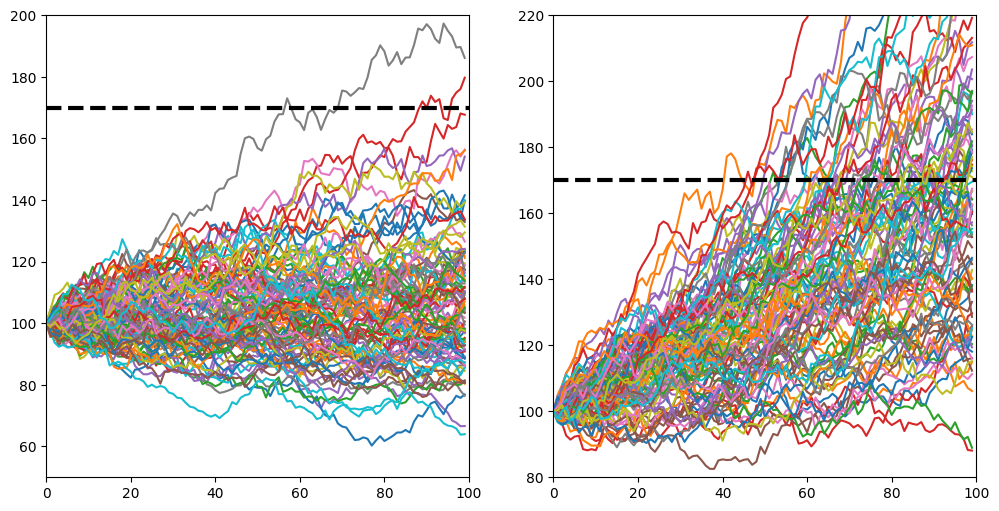
\includegraphics[width=0.85\textwidth]{figures/importance_sampling_5}
	\caption{Distribution of GBM paths (left) with real drift term, (right) with adjusted drift term.}
	\label{fig:importance_sampling_5}
\end{figure}

There is a clear connection between importance sampling and Radon-Nikodym derivative (or Girsanov theorem):
\begin{equation}
	\begin{gathered}
		\mathbb{E}[f(x)] = \int f(x)p(x) dx = \int f(x) \cfrac{p(x)}{q(x)} dx\\
		\mathbb{E}^{\mathbb{Q}}[f(S_T)]= \mathbb{E}^{\mathbb{Q}_0}\left[f(S_T)\cfrac{d\mathbb{Q}}{d\mathbb{Q}_0}\right]
	\end{gathered}
\end{equation}

The importance sampling adjustment that insures that the estimator continues to be an unbiased estimator of the option price is the ratio of the two probability densities (likelihood ratio).
So we can simulate events under $\mathbb{Q}_0$ and the multiply by the Radon-Nikodym derivative. So we get
\begin{equation}
	\begin{gathered}
		\mathbb{E}^{\mathbb{Q}}[e^{-rT}(S_0 e^{Z_T} - K)^+], \text{ where } Z_T\sim \mathcal{N}((r-\cfrac{\sigma^2}{2})T, \sigma^2T) \\
		\mathbb{E}^{\mathbb{Q}_0}[e^{-rT}(S_0 e^{Z_T} - K)^+], \text{ where } Z_T\sim \mathcal{N}(\mu T, \sigma^2T)
	\end{gathered}
\end{equation}

We would like to determine the \emph{optimal} $\mu$ such that the variance is minimized. Unfortunately there is not straightforward way to do that. One can try to determine a relatively optimal value by
\begin{equation}
\min_{\mu}\mathbb{E}^{\mathbb{Q}}\left[f^2(x)\cfrac{p(x)}{q_\mu(x)}\right]
\end{equation}

\begin{ipythonnon}
from scipy.stats import norm
from scipy.optimize import fmin, minimize

def Q0(mu, x, sigma, T):
	return norm(mu*T, sigma*T).pdf(x)

def Q(x, r, sigma, T):
	return norm((r - 0.5*sigma**2)*T, sigma*T).pdf(x)

def f(x, r, S0, K):
	return np.exp(-r*T)*np.maximum(0, S0*np.exp(x) - K)

M = 1000000
def arg_min(x, mu, sigma, T):
	x_T = np.random.normal(size=M)
	z = (mu - 0.5*sigma**2)*T + sigma*x_T*np.sqrt(T)
	return np.mean(f(z, mu, S0, K)**2*Q(z, mu, vol, T)/Q0(x, z, vol, T))

res = minimize(arg_min, 0.6, args=(mu, vol, T), method='Nelder-Mead',
               options={'maxiter':2000})
print (res)
mu_star = res.x	
\end{ipythonnon}
\begin{ioutput}
message: Optimization terminated successfully.
success: True
status: 0
fun: 0.012807191452145612
x: [ 6.295e-01]
nit: 10
nfev: 26
final_simplex: (array([[ 6.295e-01], [6.296e-01]]), 
                array([ 1.281e-02,  1.287e-02]))
\end{ioutput}

So we can check how importance sampling works with different number of samples. ranging from 100 to 50000, see Fig.~\ref{fig:importance_sampling_6}.

\begin{ipythonnon}
np.random.seed(1)
C0_is, SE_is = [], []
C0_wo, SE_wo = [], []

Ms = [100, 500, 1000, 2500, 5000, 10000, 25000, 50000]
for M in Ms:
	x_T = np.random.normal(size=M)
	z = mu_star*T - vol*x_T*np.sqrt(T)
	C_is = f(z, mu, S0, K)*Q(z, mu, vol, T)/Q0(mu_star, z, vol, T)

z = (mu-0.5*vol**2)*T + vol*x_T*np.sqrt(T)
C_wo = f(z, mu, S0, K)
C0_is.append(np.mean(C_is))
SE_is.append(np.std(C_is))
C0_wo.append(np.mean(C_wo))
SE_wo.append(np.std(C_wo))

data = pd.DataFrame({"M":Ms, "DP_wo":C0_wo, "DP_is":C0_is, "std_wo":SE_wo,
                     "std_is":SE_is})
data['reduction'] = data['std_wo']/data['std_is']
print (data.head(20))
\end{ipythonnon}
\begin{ioutput}
       M     DP_wo     DP_is    std_wo    std_is  reduction
0    100  0.000000  0.088340  0.000000  0.085636   0.000000
1    500  0.156567  0.074716  2.661602  0.082478  32.270467
2   1000  0.072207  0.080365  1.183912  0.085448  13.855288
3   2500  0.090879  0.078064  1.512354  0.083297  18.156072
4   5000  0.106882  0.079540  1.624668  0.084151  19.306581
5  10000  0.071713  0.078611  1.308213  0.083662  15.636928
6  25000  0.079021  0.078641  1.238422  0.083380  14.852823
7  50000  0.083900  0.078832  1.343988  0.083419  16.111264
\end{ioutput}

\begin{figure}[htb]
	\centering
	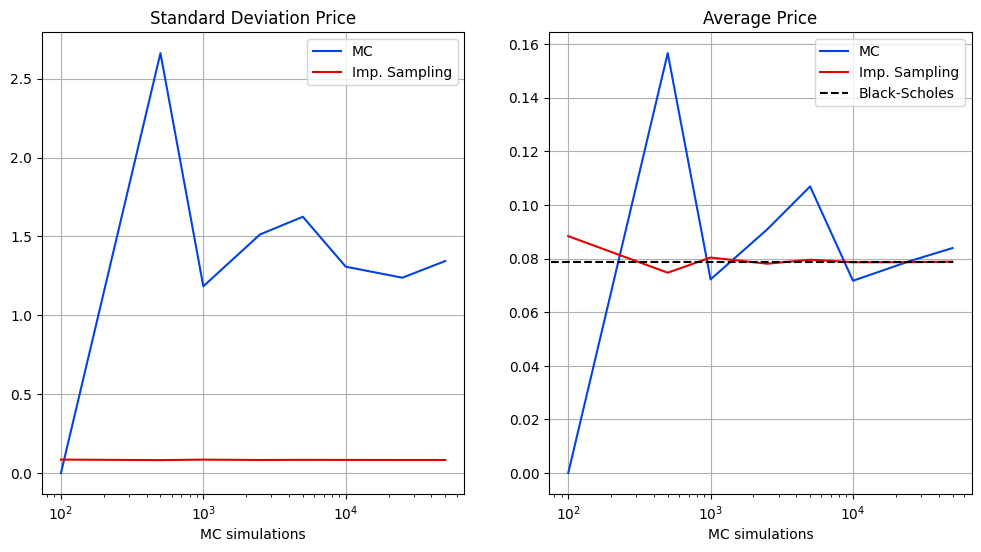
\includegraphics[width=0.8\textwidth]{figures/importance_sampling_6}
	\caption{Convergence of the importance sampling technique compared to "raw" Monte Carlo as a function of the number of simulations. It is apparent how the variation reduction technique dramatically improves
	the result.}
	\label{fig:importance_sampling_6}
\end{figure}

\subsection{Variation Reduction Techniques Comparison}
There is a common misconception that Importance Sampling (IS) is always the "strongest" technique. In reality, IS is a specialized tool, whereas Control Variates (CV) and Antithetic Variates
(AV) are general-purpose tools.

Indeed comparing the results of the previous examples turns out that IS is not the best method, this conclusion can be due to the following issue.
Importance Sampling is designed to solve one specific problem: \emph{rare events}.
Considering again the European option case we may have two possibilities. If $S_0=100$ and $K=100$, the option is at-the-money and it has a 50\% chance of finishing in the money. Standard MC is already very good here. If you use IS, you are "forcing" the math to look at something it already sees clearly, often adding noise via the likelihood ratio.
If instead $S_0=100$ but $K=180$ (deep out-of-the-money), the option only finishes in the money 1\% of the time. Standard MC will give you zeros for 99\% of paths (huge variance). This is where IS wins, 
because it forces the simulation to look at that 1\% area.

In IS, your estimator is: $\text{Payoff}\times \text{Likelihood Ratio}$; with the likelihood ratio being an exponential function. Exponential functions have very high variance so
\begin{itemize}
	\item In Antithetic, you are averaging two correlated payoffs. This smooths the data.
	\item  In Control Variates, you	are subtracting known error. This anchors the data.
	\item In Importance Sampling, you are multiplying the payoff by a volatile weight. If your shift ($\mu_{shift}$) is too aggressive, the weight can explode or vanish, increasing the intrinsic standard deviation of the samples.
\end{itemize} 

%%This section implements a Monte Carlo simulation to price a European call option using the importance sampling technique for variance reduction.
%%	
%%	\textbf{Note on the original MATLAB code:} The provided MATLAB code for
%%	importance sampling contained some issues in the calculation of the
%%	likelihood ratio (\texttt{is\_ratio}) and the final estimator.
%%	Specifically, \texttt{VY\ =\ A\_is\ +\ B*n;} incorrectly used \texttt{n}
%%	(number of paths) instead of a random variable, and the
%%	\texttt{is\_ratio} and final \texttt{E\_is} calculations did not follow
%%	the standard importance sampling methodology. The
%%	\texttt{normfit(DiscPayoff.*ISRatios)} also referred to undefined
%%	variables and an inappropriate function for simply getting the mean/std.
%%	
%%The Python code below implements a standard and correct importance sampling approach, where we shift the mean of the underlying normal distribution to focus sampling efforts on the region where the option
%%has a non-zero payoff (i.e., where \(S_T > K\)). We then adjust the	payoffs by the likelihood ratio (Radon-Nikodym derivative) to ensure the estimator remains unbiased.
%%	
%%Yes, this code is mathematically and logically correct for implementing	Importance Sampling (IS) in the Black-Scholes framework.
%%	
%%You have correctly applied the Change of Measure (Girsanov Theorem simplified for the normal distribution). By shifting the mean of Z, you are forcing the simulation to generate more ``In-The-Money'' (ITM)
%%paths, which are the ones that actually contribute to the option's value. Why the Math is Correct 1. The Shift (μshift\hspace{0pt})
%%	
%%You chose μshift\hspace{0pt} such that the ``average'' simulated price ST\hspace{0pt} ends up exactly at the strike K.
%%	
%%\begin{verbatim}
%%In standard Monte Carlo, if an option is Out-of-the-Money (OTM), most paths result in a payoff of 0. This is "wasted" computation.
%%		
%%By shifting the distribution, you ensure that roughly 50% of your paths end up ITM, providing more "information" to the estimator.
%%\end{verbatim}
%%	
%%	\begin{enumerate}
%%		\def\labelenumi{\arabic{enumi}.}
%%		\setcounter{enumi}{1}
%%		\tightlist
%%		\item
%%		The Likelihood Ratio (Radon-Nikodym Derivative)
%%	\end{enumerate}
%%	
%%When you change the distribution from P to Q, you must multiply the	result by the likelihood ratio L=dQdP\hspace{0pt} to keep the estimator unbiased. For a shift in a normal distribution N(0,1)→N(μ,1), the ratio
%%is: L(Z)=exp(−μZ+21\hspace{0pt}μ2)
%%	
%%(Note: Your code uses - 0.5 * mu\_shift**2, which is correct because you are evaluating it using the original samples Z before the shift was applied). 
%%In your code, you use Z\_original\_samples to calculate the	likelihood\_ratio. While correct, it can be confusing because the likelihood ratio is usually expressed in terms of the samples used in
%%the payoff (Zshifted\hspace{0pt}).
%%	
%%If you rewrite it using the actual samples that went into ST\hspace{0pt}: \# Likelihood ratio using the samples that were actually shifted 
%%likelihood\_ratio = np.exp(-mu\_shift * Z\_shifted\_samples + 0.5 * mu\_shift**2)
%%	
%%This is mathematically identical to your version but matches the standard textbook formula for the Radon-Nikodym derivative more closely.
%%	
%%\begin{Verbatim}[commandchars=\\\{\}]
%%Estimated European Call Option Price (IS): 10.4063
%%Standard Deviation of Price Estimate (IS): 17.5629
%%\end{Verbatim}



